\documentclass[letter]{ieicej}
\usepackage{graphicx}
%\usepackage{latexsym}
%\usepackage[fleqn]{amsmath}
%\usepackage[psamsfonts]{amssymb}

\setcounter{page}{1}

\typeofletter{研究速報}
%\typeofletter{紙上討論}
%\typeofletter{問題提起}
%\typeofletter{ショートノート}
\field{}
\jtitle{ダイジェスト視聴可能なP2Pライブストリーミングの提案}
\etitle{Proposal and Evaluation of P2P live streaming system for digest viewing}

\authorlist{
  \authorentry[shunsuke@spa.is.uec.ac.jp]{鈴木 駿介}{Shunsuke SUZUKI}{s}{UEC}%
  \authorentry[]{末田 欣子}{Yoshiko SUEDA}{m}{UEC,NTT}%
  \authorentry[]{多田 好克}{Yoshikatsu TADA}{m}{UEC}%
}
\affiliate[UEC]{電気通信大学 大学院情報システム学研究科\hskip1zw〒182-8585 東京都調布市調布ケ丘1--5--1}{Guraduate School of Information Systems,The University of Electro-Communications\hskip1em1--5--1, Chofugaoka, Chofu-shi, Tokyo, 182--8585 Japan}
\affiliate[NTT]{日本電信電話株式会社 NTTネットワーク基盤技術研究所\hskip1zw〒180-0012 東京都武蔵野市緑町3--9--11}{NTT Network Technology Laboratories,Nippon Telegraph and Telephone Corporation\hskip1em3--9--11, Midori-Cho, Chofu-shi, Tokyo, 180--8585 Japan}
%\affiliate[所属ラベル]{和文所属}{英文所属}
%\paffiliate[]{}
%\paffiliate[現在の所属ラベル]{和文所属}

\begin{document}
\maketitle
\begin{abstract}
  P2P(peer to peer)におけるライブストリーミングは配信者への負荷の集中を軽減できたり, サーバ-クライアント方式よりも低コストで実現できるなど, 近年その需要は高まっている. しかし, 既存のP2Pライブストリーミングシステムでは, 途中参加したユーザはそれまでの配信内容を把握することができないといった問題がある. そのため, P2Pライブストリーミングにおいて, 途中参加したユーザがダイジェストを視聴可能なP2Pライブストリーミングシステムが必要となる. 本研究では, そのようなP2Pライブストリーミングシステムにおいて, P2Pネットワーク内でダイジェストを作成し, 保持し, 広めるために各ピアが役割を持ったトポロジを提案する. シミュレーションの結果, ノード数が増加してもネットワーク全体のスループットは低下しなかった. さらに, 役割を持たせなかった場合と比べ役割を持たせた場合は全体的なスループットが大きく, 役割を与えることの有用性を確認することが出来た.
\end{abstract}
\begin{keyword}
  P2P, ダイジェスト, トポロジ, 役割
\end{keyword}
\begin{eabstract}
  Live streaming in P2P(peer to peer) can solve a concentration of load on a distributor, and its demand has increased in recent years. But, users joined since live streaming starts unable to understand the content of a distribution in the existing method. Threfore, a live streaming system that users joined since live streaming starts can watch digests is required. In this study, we propose new topology that peers have roles of creating, keeping and spreading digests in P2P network for such  P2P live streaming. As a result of simulation, when the number of peers so increased, the throughput of network did not decrease. We show the peers having role are higher throughput than the peers having not role.
\end{eabstract}
\begin{ekeyword}
  P2P, digest, topology, role
\end{ekeyword}

\section{背景}
ネットワーク技術の発達に伴い, ネットワークを用いた動画配信サービスが急速に普及している. 特にニコニコ生放送\cite{nico}やUSTREAM\cite{ust}といったリアルタイム動画配信サービスが人気である. 動画配信の形態としてはサーバ-クライアント方式が一般的であるが, 配信サーバのコスト削減や配信者の負荷を軽減するためP2Pを利用したライブストリーミング配信が期待されている.

P2Pライブストリーミングは主にアプリケーションレベルマルチキャスト(ALM: Application Level Multicast)によって行われる. ALMはアプリケーションによって実現されるため開発が容易で多くの研究がなされている.

ALMは主にツリー型とメッシュ型に分類される. ツリー型は遅延が少なく構築が容易であるというメリットがあるが, 耐故障性やノードの離脱に弱いといったデメリットがある. メッシュ型は耐故障性やノードの離脱に強いというメリットがあるが, 複数の経路を用いるため遅延が大きくなるといったデメリットがある. 一方でこれらツリー型やメッシュ型の欠点を補うために複数クラスタ型\cite{dis},\cite{streamline}が提案されている. 複数クラスタ型は複数のクラスタを構築し各サブストリームをそれぞれのクラスタで配信するといった方法である. 複数クラスタ型ではツリー構造のように中継ノードにストリームを渡すため, 配信の負荷が軽減される. またクラスタ内部では各ノードが複数の経路を持つため耐故障性に優れる.

また, 動画配信サービスにおいてダイジェストを見ることは, 動画全体の雰囲気を知るために有用である. リアルタイム動画配信であるライブストリーミングにおいても, 途中から配信に参加した場合にそれまでの配信の内容を把握出来るという点においてダイジェストを見ることは有用である. しかし, P2Pのライブストリーミングにおいては, ダイジェストを保存しておくサーバを用意することが出来ないなどの問題がある. また, 野球など特定のスポーツ映像にのみ対応可能なダイジェスト生成方式\cite{bb}, \cite{sport}などもあるが, 様々な内容の動画配信に対応させることは難しい.

そこで本研究では, 配信に途中参加したユーザがダイジェスト視聴可能なP2Pライブストリーミングシステムにおいて, P2Pネットワーク内でダイジェストを生成し, 保持し, 広めるために各ピアが役割を持ったトポロジを提案する. ダイジェストを作成する専用のサーバは設置せず, ネットワーク内に存在するピアが作成し, それをネットワーク内に広める. システムはダイジェストがP2Pネットワーク内で枯渇しないような設計にする必要がある.

\section{関連研究}
\subsection{階層型クラスタ構造}
Yang Guoらは階層的クラスタHCPS\cite{hcps}を提案している. HCPSはクラスタ間で帯域のバランスを取ることにより, より品質の高い映像を流すことを可能にしている. クラスタ内部は完全結合となっており, 各クラスタのアップロード容量が均一になるように構成されている. ヘッドノードのアップロード容量は大きくなっている.

HCPSはクラスタの中身が完全結合のため各ノードへのホップ数や遅延が多くなってしまうという課題がある.

\begin{figure}[h]
  \begin{center}
    \includegraphics{fig1.eps}
  \end{center}
  \caption{階層型クラスタのP2Pライブストリーミング}
  \label{fig:fig01}
  \ecaption{A hierarchical cluster in P2P live streaming}
\end{figure}

\subsection{重畳クラスタ木型動画配信システム}
元橋らは重畳クラスタ木方式の動画配信システム\cite{chojo}を提案している. 階層的なクラスタ構造になっており, クラスタ間の配信木の中継ノードであるゲートノードが存在する. ゲートノード選出方式として, 滞在時間の長さとRTTを考慮した方法を提案している. 離脱耐性向上型, 配信遅延抑制型, ハイブリッド型の実験をしたところ, ハイブリッド型が最も性能が良いという結果が出ている.

重畳クラスタ木方式は全体として木構造のため下位のクラスタほど配信者からのホップ数が大きくなってしまうという課題がある.

\begin{figure}[h]
  \begin{center}
    \includegraphics{fig2.eps}
  \end{center}
  \caption{階層型のストライプ配信}
  \label{fig:fig02}
  \ecaption{A striped broadcast}
\end{figure}

\subsection{ハイブリッドアーキテクチャ構造}
Huey-Ing Liuらは局所性と貢献度を考慮したハイブリッドアーキテクチャであるMeTree\cite{metree}を提案している. これはツリー構造とメッシュ構造のハイブリッドである. 貢献度の高いピアには質の高い映像を配信し, 貢献度の低いピアには質の低い映像を配信する. 異なる貢献度を持つピアに異なるQoE(Quality of Experience)を与えているが, それ故ネットワーク全体のQoEは低下してしまう.

MeTreeでは貢献度を意識した設計のため貢献度の低いノードは良い映像が見られずネットワーク全体のQoEは低下してしまうという課題がある.

\begin{figure}[h]
  \begin{center}
    \includegraphics{fig3.eps}
  \end{center}
  \caption{MeTree}
  \label{fig:fig03}
  \ecaption{MeTree}
\end{figure}

\newpage

\section{提案システム}
本研究の目的は, 配信に途中参加したユーザがダイジェスト視聴可能なP2Pライブストリーミングシステムにおいて, P2Pネットワーク内でダイジェストを生成し, 保持し, 広めるために各ピアが役割を持ったトポロジを設計することである. 本研究の要求条件の1つは遅延や離脱耐性を考慮した階層型クラスタにすることである. もう1つの要求条件はネットワーク内のダイジェストを枯渇させないことである. 要求条件を達成するためにクラスタ内部の論理ホップ数は少なくなるように配置する. またダイジェストはクラスタ内ですべての種類が揃っているようにする. こうすることでダイジェストを取得するまでの論理ホップ数を軽減させることが出来る.

\subsection{配信内容に対するコメント}
本研究で提案するP2Pライブストリーミングシステムでは, 参加ユーザが配信内容に対して自由にコメント投稿が出来ることを想定する. コメントは1ユーザにつき何回でも投稿出来るものとする. 各ユーザが投稿したコメント数はシステム内で管理し, 各ノードの役割を決定するために指標として利用する.

\subsection{ノードの役割}
3つの役割を各ノードに与える.

ゲートノード: 配信者ノードから受け取ったストリームの情報をクラスタ内で一番最初に受取り, それを広める役割を担う. これは配信者ノードの負担を軽減し, 素早くクラスタ内に広めるために必要である. 高帯域でコメント数の多いピアが選ばれる.

セミゲートノード: ゲートノードから受け取ったデータをクラスタ内に広める役割を担う. さらにゲートノードが離脱した場合には即座にこのピアがゲートノードの代わりになることを考えている. ゲートノードの次に高帯域でコメント数の多いピアが選ばれる.

ダイジェストノード: ダイジェストを保有し, 新規参加ノードに渡す役割を担っている. コメント数が多いピアが選ばれる. これはコメント数の多いピアは離脱耐性が低いと考えられ, ダイジェストの枯渇を防ぐ狙いがある.

また, トラッカーサーバを用いることとする. 各ノードのコメント数や帯域幅は常にトラッカーサーバが計算し, 管理する.

\subsection{ノードの役割決定方法}
ノードの役割はダイジェストノード, ゲートノード, セミゲートノード, ノーマルノードの順番で決定する. まずダイジェストノードはコメント数の多い全ノードの上位20\%を選択する. その後ゲートノードは, 全ノードからダイジェストノードを除いたうち帯域幅上位10\%を選択する. そしてセミゲートノードは, 全ノードからダイジェストノードとゲートノードを除いたうち帯域幅上位10\%〜20\%を選択する. 最後にノーマルノードは, 全ノードからダイジェストノードとゲートノードとセミゲートノードを除いたノードとする.

\subsection{ノード間の接続方法}
まず, クラスタ外部での接続方法を示す. 配信者ノードは全てのゲートノードと接続する. 1つのゲートノードは他のクラスタのゲートノード1つずつと接続することとする.

次にクラスタ内部での接続方法を示す. 1つのゲートノードは他の全てのゲートノードと接続する. また対応するセミゲートノード1つずつと接続する. 1つのセミゲートノードはダイジェストノードの3分の1と接続する. またノーマルノード2つずつと接続する. 1つのダイジェストノードはダイジェスト未取得ノーマルノード全てと接続する. ノーマルノードはノーマルノードの4分の1と接続することとする.

\subsection{提案するトポロジの全体イメージ図}
提案するトポロジの全体イメージを図\ref{fig:fig04}に示す. 配信者ノードから各クラスタのゲートノードにストリームの情報を送り, 各ゲートノードがその情報をクラスタ内に広める.

\begin{figure}[h]
  \begin{center}
    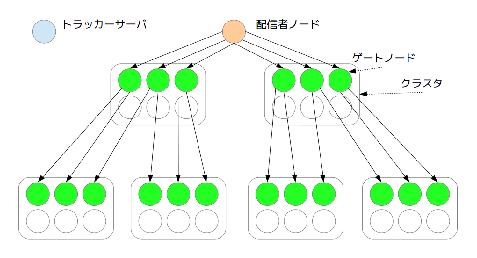
\includegraphics{fig4.eps}
  \end{center}
  \caption{提案するトポロジ全体イメージ図}
  \label{fig:fig04}
  \ecaption{The whole image of our proposal topology}
\end{figure}

クラスタの内部構造を図\ref{fig:fig05}に示す. 図\ref{fig:fig05}は図\ref{fig:fig04}における枠で囲ったクラスタ部分の詳細イメージである.

\begin{figure}[h]
  \begin{center}
    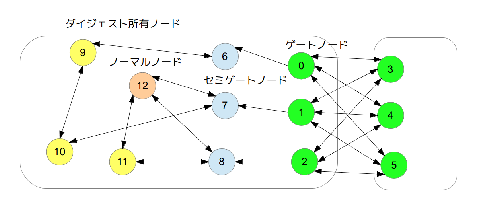
\includegraphics{fig5.eps}
  \end{center}
  \caption{提案するクラスタ構造}
  \label{fig:fig05}
  \ecaption{The clustering structure of our proposal system}
\end{figure}

\subsection{新規参加ピア}
新規参加ピアの行動について述べる. 新規参加ピアはネットワーク接続時に配信者ノードにつなぐ. その後, トラッカーサーバが新規参加ピアの帯域や各クラスタへの論理ホップ数を計算し, 最も論理ホップ数の小さいクラスタに配置される(もしくはRTTの小さいクラスタに配置される). クラスタに配置された後, ダイジェスト保有ピアからダイジェストを受け取り, ダイジェストの映像を見ることが出来る.

\subsection{再構築のタイミング}
再構築のタイミングは3つある. 1つ目は新規参加ピアがダイジェストを取得し終わった時である. ダイジェスト保有ノードと接続を切断したあと, 帯域に応じて接続数を決定する. 帯域が十分に高い場合にはセミゲートノードになる. 2つ目はコメント数が一定数を超えた時である. この場合, 対象のノードはダイジェスト保有ノードになる. 3つ目はノードが離脱した時である. 離脱ノードに接続していたピアは帯域に応じた接続数を維持するように他のピアと接続する. 特にゲートノードが離脱した場合はセミゲートノードが即座にゲートノードになる. また, 特にセミゲートノードが離脱した場合はクラスタの中で帯域が高いピアがセミゲートノードになる.

\subsection{トポロジの設計の比較}
既存のトポロジ設計との比較を表\ref{tb:tb1}に示す.

\begin{table}[h]

  \centering

  \vspace*{0.3cm}
  \caption{既存システムと提案システムの比較 \label{tb:tb1}}
  \ecaption{Comparison with existing systems and our proposal system}
  \begin{tabular}{|c|c|c|c|c|} \hline
    & HCPS & 重畳 & MeTree & 提案 \\ \hline
    \shortstack{ダイジェ \\ スト} & なし & なし & なし & あり\\ \hline
    クラスタ & \shortstack{完全 \\ 結合} & \shortstack{一部 \\ メッシュ} & \shortstack{一部 \\ メッシュ}  & \shortstack{一部 \\ メッシュ}\\
    \hline
    \shortstack{ゲート \\ ノード} & \shortstack{高帯域 \\ ピア} & \shortstack{滞在時間 \\ の長い \\ ピア} & \shortstack{高帯域 \\ ピア} & \shortstack{高帯域+ \\ コメント \\ 量の多い \\ ピア} \\
    \hline
  \end{tabular}
\end{table}

\section{シミュレーション}
\subsection{前提条件}
シミュレーションを行うにあたっての前提条件について示す. 全ノードには固有の帯域幅を割り当てる. 表\ref{tb:tb2} にそれを示す.

\begin{table}[h]

  \centering

  \vspace*{0.3cm}
  \caption{帯域幅分布 \label{tb:tb2}}
  \ecaption{Bandwidth distribution}
  \begin{tabular}{|c|c|c|c|c|c|c|c|c|c|c|} \hline
    \shortstack{帯域幅 \\ (kbps)} & 256 & 320 & 384 & 448 & 512 & 640 & 768 & 1024 & 1500 & 3000 \\ \hline
    \shortstack{割合 \\ (\%)} & 10.0 & 14.3 & 8.6 & 12.5 & 2.2 & 1.4 & 6.6 & 28.1 & 1.4 & 14.9 \\ \hline
  \end{tabular}
\end{table}

また全ノードには固有のコメント数を割り当てる. サンプルとして1つの動画に対して分析を行った結果を利用する\cite{comment}. 平均コメント数は4で標準偏差は6.8である. 分析の結果を図\ref{fig:fig06}に示す.

\begin{figure}[h]
  \begin{center}
    \includegraphics{fig6.eps}
  \end{center}
  \caption{コメント数分析の結果}
  \label{fig:fig06}
  \ecaption{Result of number of comments analysis}
\end{figure}

固有のコメント数を割り当てた結果を表\ref{tb:tb3}に示す.

\begin{table}[h]

  \centering

  \vspace*{0.3cm}
  \caption{コメント数分布 \label{tb:tb3}}
  \ecaption{Number of comments distribution}
  \begin{tabular}{|c|c|c|c|c|c|c|c|c|c|c|} \hline
    \shortstack{コメント数} & 2 & 5 & 7 & 10 & 12 & 15 & 17 & 20 & 22 & 25 \\ \hline
    \shortstack{割合 \\ (\%)} & 16 & 17 & 17 & 16 & 15 & 13 & 10 & 2 & 1 & 1 \\ \hline
  \end{tabular}
\end{table}

全ノード数に応じたクラスタの数を予め設定する. 全ノード数とクラスタ数対応表を表\ref{tb:tb4}に示す.

\begin{table}[h]

  \centering

  \vspace*{0.3cm}
  \caption{ノード数とクラスタ数対応表 \label{tb:tb4}}
  \ecaption{Number of nodes and clusters distribution}
  \begin{tabular}{|c|c|c|c|c|} \hline
    \shortstack{ノード数} & 200 & 400 & 600 & 800 \\ \hline
    \shortstack{クラスタ数} & 7 & 10 & 14 & 18  \\ \hline
  \end{tabular}
\end{table}

その他の前提条件として, ノード間遅延を全てのノード間で100msに設定している. またパケットロス率は0\%として考慮しないこととする.

\subsection{結果}
シミュレーションで用いたトポロジの例を図\ref{fig:fig07}に示す. この例ではノード数を200とし, クラスタを7としている. 配信者ノードは1, ゲートノードは21, セミゲートノードは21, ダイジェストノードは42, ダイジェスト取得済ノーマルノードは84, ダイジェスト未取得ノーマルノードは28でそれぞれ分布している.

\begin{figure}[h]
  \begin{center}
    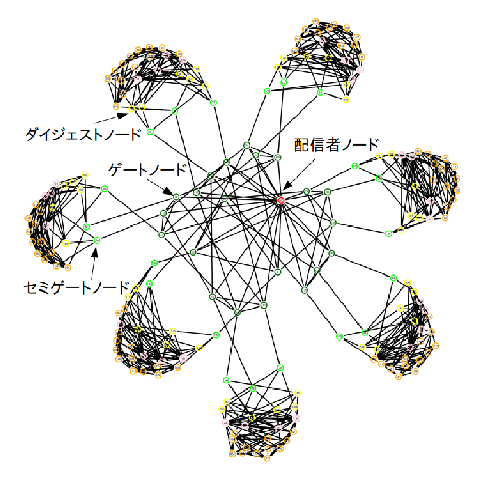
\includegraphics{topology.eps}
  \end{center}
  \caption{提案するトポロジ(200ノード)}
  \label{fig:fig07}
  \ecaption{Proposal topology(200 nodes)}
\end{figure}

図\ref{fig:fig08}と図\ref{fig:fig09}は各ノード数におけるスループット推移の様子である. また図\ref{fig:fig10}はスループットの推移の平均を示している. 他のノード数と比較してノード数が200の時にスループットが低下しているが, ノード数が大きくなってもスループットの低下は見られないことがわかる.

\begin{figure}[h]
  \begin{center}
    \includegraphics{fig8.eps}
  \end{center}
  \caption{各ノード数におけるスループット推移の様子}
  \label{fig:fig08}
  \ecaption{Throughput versus node number}
\end{figure}

\begin{figure}[h]
  \begin{center}
    \includegraphics{fig9.eps}
  \end{center}
  \caption{各ノード数におけるTCP通信を含めたスループット推移の様子}
  \label{fig:fig09}
  \ecaption{Throughput versus node number including TCP}
\end{figure}

\begin{figure}[h]
  \begin{center}
    \includegraphics{fig10.eps}
  \end{center}
  \caption{各ノード数におけるスループット推移の様子の平均}
  \label{fig:fig10}
  \ecaption{Average throughput versus node number}
\end{figure}

さらに役割を与えた場合と与えない場合との比較を行う. ノード数とクラスタ数の対応は表\ref{tb:tb4}に従うものとする. また役割に関しては, ゲートノード, セミゲートノード, ダイジェストノードを廃止して全てのノードがノーマルノードになるようにする. 配信者ノードからは各クラスタに1つずつ繋がるようにする. 図\ref{fig:fig11}は役割を与えなかった場合のトポロジの例を示している. この例ではノード数を200とし, クラスタを7としている.

\begin{figure}[h]
  \begin{center}
    \includegraphics{topology2.eps}
  \end{center}
  \caption{役割を与えない場合のトポロジ}
  \label{fig:fig11}
  \ecaption{Topology in case of no role}
\end{figure}

図\ref{fig:fig12}と図\ref{fig:fig13}は役割を与えない場合の各ノード数におけるスループット推移の様子である. ノード数が大きい場合にスループットが低下している様子がわかる.

\begin{figure}[h]
  \begin{center}
    \includegraphics{fig12.eps}
  \end{center}
  \caption{役割を与えない場合の各ノード数におけるスループット推移の様子}
  \label{fig:fig12}
  \ecaption{Throughput versus node number in case of no role}
\end{figure}

\begin{figure}[h]
  \begin{center}
    \includegraphics{fig13.eps}
  \end{center}
  \caption{役割を与えない場合の各ノード数におけるTCP通信を含めたスループット推移の様子}
  \label{fig:fig13}
  \ecaption{Throughput versus node number incase of no role including TCP}
\end{figure}

図\ref{fig:fig15}は役割を与えた場合と与えない場合のノード数におけるスループットの推移の様子の平均の比較を示している. ノード数が大きくなるに連れて, 役割を与えない場合はスループットが低下しているのに対し役割を与えた場合はスループットが低下していないことがわかる. さらに役割を与えたほうが全体的なスループットの値が大きく, 役割を与えることの有用性が高いことがわかる.

\begin{figure}[h]
  \begin{center}
    \includegraphics{fig15.eps}
  \end{center}
  \caption{役割を与えた場合と与えない場合の各ノード数におけるスループット推移の様子の平均の比較}
  \label{fig:fig15}
  \ecaption{Comparison with average of throughput in case of role and no role}
\end{figure}

\subsection{要求条件の達成度}
要求条件の1つは, 遅延や離脱耐性を考慮した階層型クラスタにすることであった. シミュレーションで観測できたものはスループットの様子のみであったため, 遅延や離脱耐性に対する評価が出来なかった. しかしクラスタの構築は階層型に配置することが出来た. 要求条件のもう1つは, ネットワーク内のダイジェストを枯渇させないことであった. これについても, ピアが離脱した場合などを考慮したシミュレーションを行なっていないため, 評価が出来なかった. しかし, 各クラスタにダイジェストを持つノードを配置し, クラスタ内ですべての種類のダイジェストを保持させることは出来た.

% この下に全角スペース
%%  
%% \newpage

\section{まとめ}
本研究では, 配信に途中参加したユーザがダイジェスト視聴可能なP2Pライブストリーミングシステムを提案した. トポロジ設計として階層型のクラスタ構造を提案した. さらに各ノードに役割を持たせ, ダイジェストがネットワーク内で枯渇しない設計を行った. さらにシステムは配信者から各ノード数へのホップ数を小さくし, ユーザの体感品質が高くなることを目指した.

シミュレーションの結果, 提案システムはノード数が大きくなってもスループットの低下は見られなかった. さらに役割を与えた場合と与えない場合とで比較したところ, 役割を与えた場合の方が全体としてスループットの値が大きく, 役割を与えることの有用性を確認することが出来た. しかし, 2つの要求条件を満たすシミュレーションは出来ず, 達成具合を確認することが出来なかった.

今後は, 要求条件の達成度を確認するために, 配信者ノードからの各ノードへストリームの情報が到達するまでの遅延情報や, ホップ数情報などの分析を行う予定である. さらに他のP2Pライブストリーミングシステムとの比較を行い, 本研究の有用の検証を行う予定である.


\ack %% 謝辞

%\bibliographystyle{sieicej}
%\bibliography{myrefs}
\begin{thebibliography}{99}

\bibitem{nico}
ニコニコ生放送, http://live.nicovideo.jp/.
\bibitem{ust}
USTREAM, http://www.ustream.tv/.
\bibitem{dis}
V. Padmanabhan, H. Wang, P. Chou, and K. Sripanidkulchai, “Distributing streaming me-
dia content using cooperative networking,” Proc.NOSDAV’02, pp.177–186, May 2002.
\bibitem{streamline}
G. Bianchi, N. Melazzi, L. Bracciale, F. Piccolo, and S. Salsano, “Streamline: An optimal distribution al-gorithm for peer-to-peer real-time streaming,” IEEE Trans. Parallel Distrib. Syst., vol.21, no.6, pp.857–871, June 2010.
\bibitem{bb}
熊野雅仁ら,“野球中継のハイライトシーン実時間配信を目的とした特徴のマイニングによるPCシーンの自動検出”, 映像情報メディア学会誌, vol.59, No.1, pp.77-84, 2005.
\bibitem{sport}
橋本隆子ら, ”スポーツ映像におけるシーン重要度算出アルゴリズムとその評価”, 信学会DEWS2003.
\bibitem{hcps} Yang Guo, Chao Liang, Yong Liu, “Hierarchically Clustered P2P Video Streaming: Design, implementation, and evaluation”, Computer Networks, pp.3432-3445, 2012.
\bibitem{chojo} 元橋 智紀, 藤本 章宏, 廣田 悠介, 戸出 英樹, 村上 孝三, “多様な配信木により離脱耐性と遅延抑制を向上させる重畳クラスタ木型動画配信システム”, 通信技術の革新を担う学生論文特集, p.132-142, 2014年.
\bibitem{metree} Huey-Ing Liu, その他, “MeTree: A Contribution and Locality-Aware P2P Live Streaming Architecture”, AINA 24th IEEE International Conference on, pp.1136-1143, 2010.
\bibitem{comment} “ニコニコ動画のコメントを分析してみる@2013年冬アニメ”, http://blog.livedoor.jp/mgpn/archives/51887779.html, 2014年閲覧.


\end{thebibliography}


\appendix
\section{}

\end{document}
